\begin{frame}[fragile]{disassembly issues (1)}
\begin{lstlisting}[language=myasm,style=size8]
.global main
main:
    call print_hello
    xorl %eax, %eax
    ret
.Lstr:
    .asciz "Hello!"
print_hello:
    leaq .Lstr(%rip), %rdi  // RDI <- .Lstr address
    jmp puts
\end{lstlisting}
\hrule
\begin{Verbatim}[fontsize=\fontsize{8}{9},commandchars=\\\{\}]
0000000000001139 <main>:
    1139:	e8 0a 00 00 00       	call   1148 <print_hello>
    113e:	31 c0                	xor    %eax,%eax
    1140:	c3                   	ret    
    \myemph{1141:	48                   	rex.W}
    \myemph{1142:	65 6c                	gs insb (%dx),%es:(%rdi)}
    \myemph{1144:	6c                   	insb   (%dx),%es:(%rdi)}
    \myemph{1145:	6f                   	outsl  %ds:(%rsi),(%dx)}
    \myemph{1146:	2e                   	cs}
\myemph{	...}
0000000000001148 <print_hello>:
    1148:	48 8d 3d f2 ff ff ff 	lea    -0xe(%rip),%rdi        # 1141 <main+0x8>
    114f:	e9 dc fe ff ff       	jmp    1030 <puts@plt>
\end{Verbatim}
\end{frame}

\begin{frame}[fragile]{disassembly issues}
\begin{Verbatim}[fontsize=\fontsize{8}{9},commandchars=\\\{\}]
0000000000001139 <main>:
    1139:	e8 0a 00 00 00       	call   1148 <print_hello>
    113e:	31 c0                	xor    %eax,%eax
    1140:	c3                   	ret    
    \myemph{1141:	48                   	rex.W}
    \myemph{1142:	65 6c                	gs insb (%dx),%es:(%rdi)}
    \myemph{1144:	6c                   	insb   (%dx),%es:(%rdi)}
    \myemph{1145:	6f                   	outsl  %ds:(%rsi),(%dx)}
    \myemph{1146:	2e                   	cs}
    \myemph{	...}
0000000000001148 <print_hello>:
    1148:	48 8d 3d f2 ff ff ff 	lea    -0xe(%rip),%rdi        # 1141 <main+0x8>
    114f:	e9 dc fe ff ff       	jmp    1030 <puts@plt>
\end{Verbatim}
\hrule
\begin{Verbatim}[fontsize=\fontsize{8}{9},commandchars=\\\{\}]
    1139:	e8 0a 00 00 00       	call   1148 <__cxa_finalize@plt+0x108>
    113e:	31 c0                	xor    %eax,%eax
    1140:	c3                   	ret    
    \myemph{1141:	48                   	rex.W}
    \myemph{1142:	65 6c                	gs insb (%dx),%es:(%rdi)}
    \myemph{1144:	6c                   	insb   (%dx),%es:(%rdi)}
    \myemph{1145:	6f                   	outsl  %ds:(%rsi),(%dx)}
    1146:	\myemph{2e 00} 48 8d          	cs add %cl,-0x73(%rax)
    114a:	3d f2 ff ff ff       	cmp    $0xfffffff2,%eax
    114f:	e9 dc fe ff ff       	jmp    1030 <puts@plt>
\end{Verbatim}
\end{frame}

\begin{frame}{finding assembly heuristics}
    \begin{itemize}
    \item objdump strategy, apparently:
        \begin{itemize}
        \item disassemble instructions starting at each symbol
        \item skip over strings of zero-bytes just before symbol
        \end{itemize}
    \item problem: can misidentify jumped to instructions
        \begin{itemize}
        \item especially if symbols stripped to save space/hinder reverse engineering
        \end{itemize}
    \item exercise: algorithm to fix?
        \begin{itemize}
        \item (Ghidra does this)
        \end{itemize}
    \end{itemize}
\end{frame}

\begin{frame}[fragile]{some tricky cases (1)}
\begin{Verbatim}[fontsize=\fontsize{9}{10}\selectfont]
_start:
    ...
    movq $main, %rdi
    ...
    call __libc_start_main
    ...
\end{Verbatim}
\hrule
\begin{Verbatim}[fontsize=\fontsize{9}{10}\selectfont]
struct DeviceTypeFuncs {
    void (*Send)(struct DeviceInfo*, char *);
    void (*Recv)(struct DeviceInfo, char *, size_t);
};
void SendToDevice(struct DeviceInfo* info, char *data) {
    (info->funcs->Send)(data);
}
\end{Verbatim}
\end{frame}

\begin{frame}[fragile]{some tricky cases (2)}
\begin{Verbatim}
table:
    .int case1 - table
    .int case2 - table
...

    lea table(%rip), %rax
    addq (%rax, %rdi, 4), %rax
    jmp *%rax
\end{Verbatim}
\hrule
\begin{Verbatim}
    movq $function + 0x12340, %rax
    movq $0x1234, %r9
    sll $4, %r9
    addq %r9, %rax
    call *%rax
\end{Verbatim}
\end{frame}

\begin{frame}[fragile]{some tricky cases (3)}
\begin{Verbatim}[fontsize=\small]
    call complex_func_returning_three
    lea next2-3(%rax), %rax
    jmp *%rax
    .byte 0x39, 0x59, 0x60, 0x89, 0xFF
next2:
    addq ...
\end{Verbatim}
\end{frame}


\begin{frame}
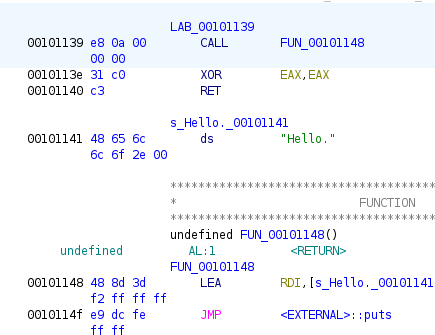
\includegraphics[height=\textheight]{../re-tools/ghidra-disass-mixed-detail}
\end{frame}
